%==============================================================
%  EE201 -- Circuit Theory I
%  Lecture 5 : The Inductor -- slides
%  M. Mert Ankaralı, METU EEE
%
%  Compile:  ./build.sh      (or: pdflatex EE201_Lecture_5_slides.tex, twice)
%  Same colour code as the handout:
%      charge = purple, current = blue, voltage = orange, power = green
%==============================================================
\documentclass[11pt,aspectratio=169]{beamer}

\usepackage[T1]{fontenc}
\usepackage[utf8]{inputenc}
\usepackage[english]{babel}
\usepackage{lmodern}
\usepackage{amsmath,amssymb}
\usepackage{booktabs}
\usepackage{array}
\usepackage{colortbl}
\usepackage{tikz}
\usepackage[american,siunitx]{circuitikz}
\usetikzlibrary{arrows.meta,positioning,calc,decorations.pathreplacing,decorations.pathmorphing,decorations.markings}
\usetikzlibrary{overlay-beamer-styles}

%-------------------- plain METU-flavoured theme --------------
\usetheme{default}
\usecolortheme{default}
\useinnertheme{rectangles}
\setbeamertemplate{navigation symbols}{}
\setbeamertemplate{itemize items}[square]
\setbeamerfont{frametitle}{size=\large,series=\bfseries}
\setbeamerfont{title}{size=\LARGE,series=\bfseries}

\definecolor{metured}{RGB}{155,27,48}
\definecolor{metugray}{RGB}{88,89,91}
\definecolor{metulight}{RGB}{243,240,241}
\definecolor{ccur}{RGB}{0,102,170}
\definecolor{cvolt}{RGB}{214,120,0}
\definecolor{cpow}{RGB}{23,128,74}
\definecolor{ccharge}{RGB}{124,60,160}
\definecolor{cflux}{RGB}{0,138,138}

\setbeamercolor{structure}{fg=metured}
\setbeamercolor{frametitle}{fg=metured,bg=}
\setbeamercolor{title}{fg=metured}
\setbeamercolor{normal text}{fg=black!88}
\setbeamercolor{block title}{fg=white,bg=metured}
\setbeamercolor{block body}{bg=metulight}
\setbeamercolor{alerted text}{fg=metured}

\setbeamertemplate{frametitle}{%
  \vspace{0.55em}%
  \usebeamerfont{frametitle}\usebeamercolor[fg]{frametitle}\insertframetitle\par
  \vspace{-0.2em}{\color{metured}\rule{\textwidth}{1pt}}\par\vspace{-0.2em}}

\setbeamertemplate{footline}{%
  \hbox{\begin{beamercolorbox}[wd=\paperwidth,ht=2.4ex,dp=1.4ex,leftskip=1.2em,rightskip=1.2em]{}%
  \tiny\color{metugray}\coursecode\ \textbar\ Lecture 5: The Inductor
  \hfill \insertframenumber/\inserttotalframenumber
  \end{beamercolorbox}}}

%-------------------- macros ----------------------------------
\newcommand{\coursecode}{EE201}
\newcommand{\term}{Fall 2026--2027}
\newcommand{\Icol}[1]{\textcolor{ccur}{#1}}
\newcommand{\Vcol}[1]{\textcolor{cvolt}{#1}}
\newcommand{\Pcol}[1]{\textcolor{cpow}{#1}}
\newcommand{\Qcol}[1]{\textcolor{ccharge}{#1}}
\newcommand{\Fcol}[1]{\textcolor{cflux}{#1}}
\newcommand{\uni}[1]{\,\mathrm{#1}}
\newcommand{\A}{\uni{A}} \newcommand{\V}{\uni{V}}
\newcommand{\W}{\uni{W}} \newcommand{\J}{\uni{J}}
\newcommand{\Cb}{\uni{C}} \newcommand{\s}{\uni{s}}
\newcommand{\Wb}{\uni{Wb}} \newcommand{\Hy}{\uni{H}}

\ctikzset{bipoles/length=0.9cm, label/align=straight,
          bipoles/vsourceam/height=0.85, bipoles/vsourceam/width=0.85}
\tikzset{
  curarr/.style={-{Stealth[length=2.6mm]}, ccur, very thick},
  blk/.style={draw=metugray, fill=metulight, rounded corners=2pt,
              minimum height=1.25cm, text width=2.45cm, align=center, font=\scriptsize},
  flowarr/.style={-{Stealth[length=3mm]}, metured, very thick},
  thru/.style={-{Stealth[length=2.2mm]}, ccur, very thick},
  acr/.style={{Stealth[length=2mm]}-{Stealth[length=2mm]}, cvolt, very thick},
  pan/.style={draw=gray!35, fill=metulight, rounded corners=3pt,
              minimum width=3.0cm, minimum height=2.3cm},
  pcap/.style={font=\scriptsize\bfseries, text=metured},
  pol/.style={font=\small, text=cvolt},
  iar/.style={-{Stealth[length=2.4mm]}, ccur, very thick},
  gnode/.style={circle, fill=metured, inner sep=0pt, minimum size=4.2pt},
  glab/.style={font=\footnotesize, text=metured},
  surf/.style={draw=cpow, very thick, dashed, rounded corners=6pt},
  gbr/.style={metugray, thick, postaction={decorate, decoration={markings,
      mark=at position 0.58 with {\arrow{Stealth[length=2.4mm]}}}}},
  vax/.style={-{Stealth[length=2mm]}, gray!70},
  crv/.style={metured, very thick},
  ttl/.style={font=\scriptsize\bfseries, text=metugray},
}

\newcommand{\ohm}{\,\Omega}
\newcommand{\Req}{R_{\mathrm{eq}}}
\newcommand{\viaxes}[3]{%
  \draw[vax] (-#1,0) -- (#1,0) node[right=1pt, font=\scriptsize, text=cvolt] {$v$};
  \draw[vax] (0,-#2) -- (0,#2) node[above=1pt, font=\scriptsize, text=ccur] {$i$};
  \node[ttl] at (0,-#2-0.68) {#3};}
\newcommand{\qvaxes}[3]{%
  \draw[vax] (-#1,0) -- (#1,0) node[right=1pt, font=\scriptsize, text=cvolt] {$v$};
  \draw[vax] (0,-#2) -- (0,#2) node[above=1pt, font=\scriptsize, text=ccharge] {$q$};
  \node[ttl] at (0,-#2-0.68) {#3};}
\newcommand{\iphiaxes}[3]{%
  \draw[vax] (-#1,0) -- (#1,0) node[right=1pt, font=\scriptsize, text=ccur] {$i$};
  \draw[vax] (0,-#2) -- (0,#2) node[above=1pt, font=\scriptsize, text=cflux] {$\varphi$};
  \node[ttl] at (0,-#2-0.68) {#3};}
\newcommand{\taxes}[4]{%
  \draw[vax] (-0.15,0) -- (#1,0) node[right=1pt, font=\scriptsize] {$t$};
  \draw[vax] (0,-#2) -- (0,#3) node[above=1pt, font=\scriptsize] {#4};}

\hypersetup{colorlinks=true,allcolors=metured}

\title{Lecture 5: The Inductor}\subtitle{the other ideal energy-storage element --- and a summary of the three}
\author{M. Mert Ankaralı}
\institute{\small Department of Electrical and Electronics Engineering\\
           Middle East Technical University}
\date{}



%==============================================================
\begin{document}

%--------------------------------------------------------------
\begin{frame}[plain]
  \titlepage
  \vspace{-1.2em}
  \begin{center}\scriptsize\color{metugray}
    \Fcol{$\blacksquare$}~flux linkage \quad \Icol{$\blacksquare$}~current \quad
    \Vcol{$\blacksquare$}~voltage \quad \Qcol{$\blacksquare$}~charge \quad
    \Pcol{$\blacksquare$}~power, energy
  \end{center}
\end{frame}

%--------------------------------------------------------------
\begin{frame}{The other way to store energy}
  \vfill
  \begin{center}
  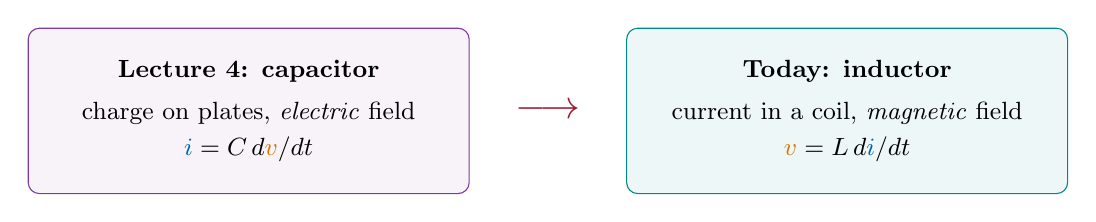
\begin{tikzpicture}[scale=1.0]
    \node[draw=ccharge, fill=ccharge!6, rounded corners=4pt, minimum width=5.6cm,
          minimum height=2.1cm, align=center, font=\small] (a) at (0,0)
         {\textbf{Lecture 4: capacitor}\\[4pt] charge on plates, \emph{electric} field\\[2pt]
          $\Icol{i} = C\,d\Vcol{v}/dt$};
    \node[draw=cflux, fill=cflux!7, rounded corners=4pt, minimum width=5.6cm,
          minimum height=2.1cm, align=center, font=\small] (b) at (7.6,0)
         {\textbf{Today: inductor}\\[4pt] current in a coil, \emph{magnetic} field\\[2pt]
          $\Vcol{v} = L\,d\Icol{i}/dt$};
    \node[font=\Large, text=metured] at (3.8,0) {$\longrightarrow$};
  \end{tikzpicture}
  \end{center}
  \vfill
  \begin{center}
    {\large The same equation with $\Vcol{v}$ and $\Icol{i}$ \alert{exchanged}.}\\[6pt]
    That is no coincidence. Try to guess each result today before it appears.
  \end{center}
  \vfill
\end{frame}

%--------------------------------------------------------------
\begin{frame}{A coil, and what it does}
  \vfill
  \begin{center}
  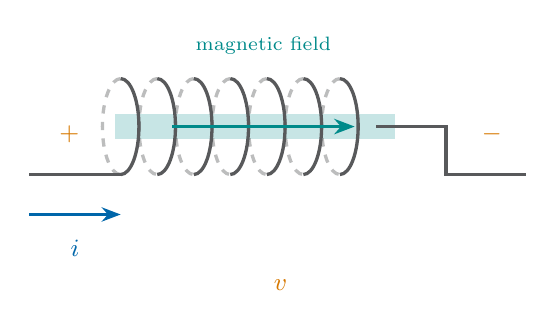
\begin{tikzpicture}[x=1.45cm, y=1.45cm]
    \draw[cflux!22, line width=9pt] (0.0,0.97) -- (2.45,0.97);
    \draw[metugray, very thick] (-0.75,0.55) -- (0.05,0.55);
    \foreach \k in {0,...,6}{
      \draw[metugray, very thick] (0.05+0.32*\k,0.55) arc (-90:90:0.16 and 0.42);
      \draw[metugray, very thick, dashed, opacity=0.40]
            (0.05+0.32*\k,1.39) arc (90:270:0.16 and 0.42);}
    \draw[metugray, very thick] (2.29,0.97) -- (2.9,0.97) -- (2.9,0.55) -- (3.6,0.55);
    \draw[iar] (-0.75,0.2) -- (0.05,0.2); \node[ccur, font=\small] at (-0.35,-0.1) {$i$};
    \draw[cflux, very thick, -{Stealth[length=2.6mm]}] (0.5,0.97) -- (2.1,0.97);
    \node[font=\scriptsize, text=cflux] at (1.3,1.68) {magnetic field};
    \node[pol] at (-0.4,0.9) {$+$};  \node[pol] at (3.3,0.9) {$-$};
    \node[pol] at (1.45,-0.42) {$\Vcol{v}$};
  \end{tikzpicture}
  \end{center}
  \vfill
  \begin{center}
    A current in the coil sets up a magnetic field running through it.\\[6pt]
    {\large The interesting part is what happens when you try to
     \alert{change} that current.}\\[8pt]
    {\small The \alert{coil} is the object on the bench.
     The \alert{inductor} is the circuit element we model it with ---
     from here on, \alert{coil} for the thing, \alert{inductor} for the element.}
  \end{center}
  \vfill
\end{frame}

%--------------------------------------------------------------
\begin{frame}{The back EMF}
  \vfill
  \begin{columns}[c,onlytextwidth]
    \begin{column}{0.21\textwidth}
      \begin{center}
      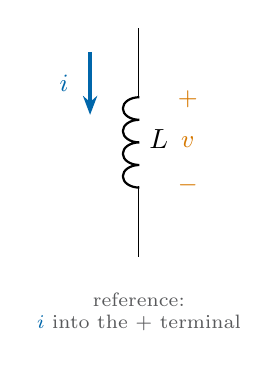
\begin{tikzpicture}[scale=1.0, transform shape]
        \draw (0,-0.45) -- (0,0) to[L, l_=$L$] (0,2.0) -- (0,2.45);
        \draw[iar] (-0.62,2.15) -- (-0.62,1.35);
        \node[ccur, font=\small] at (-0.95,1.75) {$\Icol{i}$};
        \node[pol] at (0.62,1.55) {$+$}; \node[pol] at (0.62,0.45) {$-$};
        \node[pol] at (0.62,1.0) {$\Vcol{v}$};
        \node[font=\scriptsize, text=metugray, align=center] at (0.0,-1.15)
             {reference:\\ $\Icol{i}$ into the $+$ terminal};
      \end{tikzpicture}
      \end{center}
    \end{column}
    \begin{column}{0.76\textwidth}
      \begin{center}
      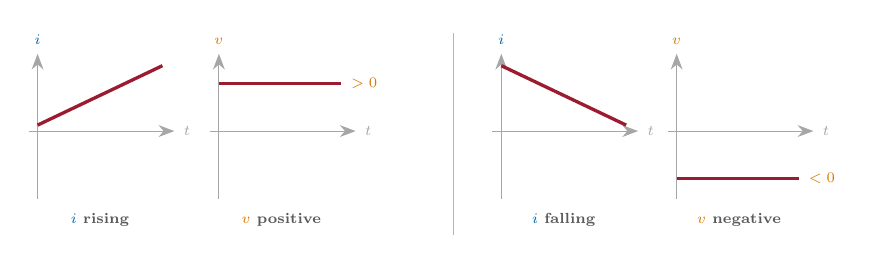
\begin{tikzpicture}[scale=0.755, transform shape]
        \begin{scope}
          \taxes{2.3}{1.15}{1.3}{\Icol{$i$}}
          \draw[crv] (0,0.1) -- (2.1,1.1);
          \node[ttl] at (1.05,-1.5) {$\Icol{i}$ rising};
        \end{scope}
        \begin{scope}[xshift=3.05cm]
          \taxes{2.3}{1.15}{1.3}{\Vcol{$v$}}
          \draw[crv] (0,0.8) -- (2.05,0.8);
          \node[font=\scriptsize, text=cvolt, right] at (2.1,0.8) {$>0$};
          \node[ttl] at (1.05,-1.5) {$\Vcol{v}$ positive};
        \end{scope}
        \draw[metugray!45] (7.0,-1.75) -- (7.0,1.65);
        \begin{scope}[xshift=7.8cm]
          \taxes{2.3}{1.15}{1.3}{\Icol{$i$}}
          \draw[crv] (0,1.1) -- (2.1,0.1);
          \node[ttl] at (1.05,-1.5) {$\Icol{i}$ falling};
        \end{scope}
        \begin{scope}[xshift=10.75cm]
          \taxes{2.3}{1.15}{1.3}{\Vcol{$v$}}
          \draw[crv] (0,-0.8) -- (2.05,-0.8);
          \node[font=\scriptsize, text=cvolt, right] at (2.1,-0.8) {$<0$};
          \node[ttl] at (1.05,-1.5) {$\Vcol{v}$ negative};
        \end{scope}
      \end{tikzpicture}
      \end{center}
    \end{column}
  \end{columns}
  \vfill
  \begin{center}
    {\large The voltage always \alert{opposes the change} that produced it ---
     the \alert{back EMF}.}\\[4pt]
    The marks never move: with $\Icol{i}$ into the $+$ terminal, a rising current makes
    $\Vcol{v}$ \alert{positive} and a falling one makes it \alert{negative}.\\[3pt]
    The faster the change, the bigger it is: $\Vcol{v} \propto d\Icol{i}/dt$.
  \end{center}
  \vfill
\end{frame}

%--------------------------------------------------------------
\begin{frame}{Inductance: how hard it pushes back}
  \vfill
  \begin{center}
    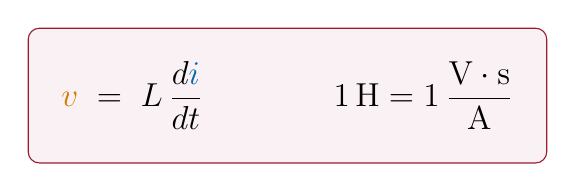
\begin{tikzpicture}
      \node[draw=metured, fill=metured!6, rounded corners=4pt, inner sep=12pt]
      {\large $\displaystyle \Vcol{v} \;=\; L\,\frac{d\Icol{i}}{dt}
        \qquad\qquad 1\Hy = 1\,\frac{\mathrm{V}\cdot\mathrm{s}}{\mathrm{A}}$};
    \end{tikzpicture}
  \end{center}
  \vfill
  \begin{center}
    One henry gives one volt of back EMF when the current rises at one ampere per second.
  \end{center}
  \vfill
  \begin{columns}[T,onlytextwidth]
    \begin{column}{0.60\textwidth}
      \begin{block}{$L$ is larger with}
        \small
        more \textbf{turns} --- each one catches the field again\\
        a different \textbf{shape} --- long and thin, or short and fat\\
        and above all what is \textbf{inside} --- iron instead of air multiplies $L$ by
        hundreds
      \end{block}
    \end{column}
    \begin{column}{0.37\textwidth}
      \begin{center}
        {\large A 1000-turn air coil,\\ $1\uni{cm}^2$, $5\uni{cm}$ long:}\\[6pt]
        {\Large\color{metured} $L \approx 2.5\uni{mH}$}\\[6pt]
        {\small nH to a few mH is normal.\\ Henries mean an iron core.}
      \end{center}
    \end{column}
  \end{columns}
  \vfill
\end{frame}

%--------------------------------------------------------------
\begin{frame}{Volt-seconds: the inductor's version of charge}
  \vfill
  \begin{center}
    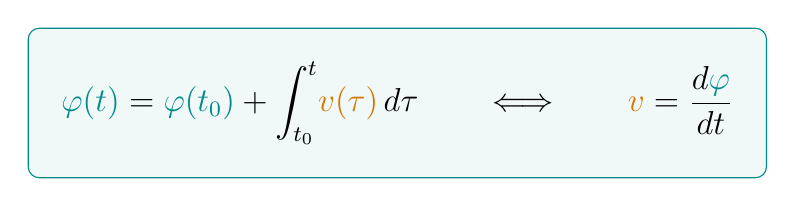
\begin{tikzpicture}
      \node[draw=cflux, fill=cflux!6, rounded corners=4pt, inner sep=12pt]
      {\large $\displaystyle \Fcol{\varphi(t)} = \Fcol{\varphi(t_0)} + \int_{t_0}^{t}\!\Vcol{v(\tau)}\,d\tau
        \qquad\Longleftrightarrow\qquad \Vcol{v} = \frac{d\Fcol{\varphi}}{dt}$};
    \end{tikzpicture}
  \end{center}
  \vfill
  \begin{center}
  \small
  \renewcommand{\arraystretch}{1.25}
  \begin{tabular}{@{}l l l@{}}
    \toprule
     & \textbf{capacitor} \footnotesize(Lecture 4) & \textbf{inductor} \footnotesize(today)\\
    \midrule
    accumulate which variable? & the current $\Icol{i}$ & the voltage $\Vcol{v}$\\
    the running total          & $\Qcol{q} = \int\!\Icol{i}\,d\tau$ & $\Fcol{\varphi} = \int\!\Vcol{v}\,d\tau$\\
    measured in                & amp-seconds $=$ coulombs & volt-seconds $=$ webers\\
    so                         & $\Icol{i} = d\Qcol{q}/dt$ & $\Vcol{v} = d\Fcol{\varphi}/dt$\\
    \bottomrule
  \end{tabular}
  \end{center}
  \vfill
  \begin{center}
    Everything in this lecture follows from that one definition.
  \end{center}
  \vfill
\end{frame}

%--------------------------------------------------------------
\begin{frame}{Why it is called \emph{flux linkage}}
  \vfill
  \begin{center}
    {\large $\Fcol{\varphi}$ is the \alert{magnetic field inside the inductor},
     counted once for every turn it passes through.}
  \end{center}
  \vfill
  \begin{center}
  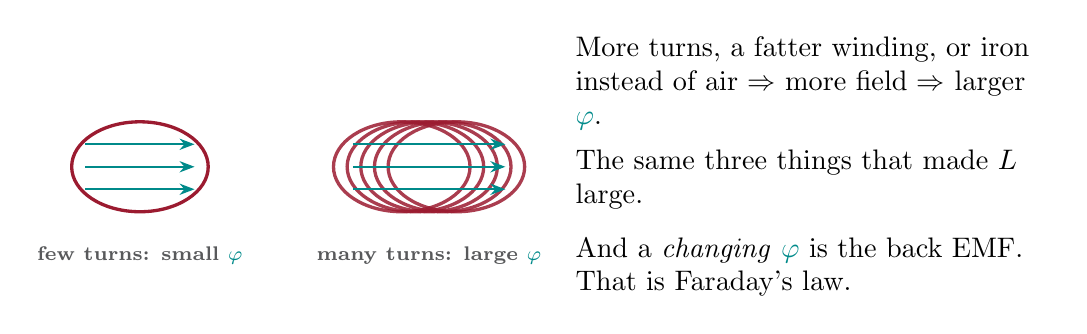
\begin{tikzpicture}[scale=1.02, transform shape]
    \begin{scope}
      \draw[metured, very thick] (0,0.1) ellipse (0.85 and 0.56);
      \foreach \dy in {-0.28,0,0.28}{
        \draw[cflux, thick, -{Stealth[length=1.9mm]}] (-0.68,0.1+\dy) -- (0.68,0.1+\dy);}
      \node[ttl] at (0,-1.0) {few turns: small $\Fcol{\varphi}$};
    \end{scope}
    \begin{scope}[xshift=3.6cm]
      \foreach \dx in {-0.34,-0.17,0,0.17,0.34}{
        \draw[metured, very thick, opacity=0.85] (\dx,0.1) ellipse (0.85 and 0.56);}
      \foreach \dy in {-0.28,0,0.28}{
        \draw[cflux, thick, -{Stealth[length=1.9mm]}] (-0.95,0.1+\dy) -- (0.95,0.1+\dy);}
      \node[ttl] at (0,-1.0) {many turns: large $\Fcol{\varphi}$};
    \end{scope}
    \node[font=\normalsize, anchor=west, text width=5.9cm] at (5.3,0.1)
      {More turns, a fatter winding, or iron instead of air $\Rightarrow$ more field
       $\Rightarrow$ larger $\Fcol{\varphi}$.\\[4pt]
       The \alert{same three things} that made $L$ large.\\[7pt]
       And a \emph{changing} $\Fcol{\varphi}$ is the back EMF. That is Faraday's law.};
  \end{tikzpicture}
  \end{center}
  \vfill
  \begin{center}
    {\small $\Qcol{q}$ is countable stuff; volt-seconds are not. Nothing piles up ---
     but $\Fcol{\varphi}$ behaves exactly as charge did.}
  \end{center}
  \vfill
\end{frame}

%--------------------------------------------------------------
\begin{frame}{What an inductor is}
  \vfill
  \begin{center}
    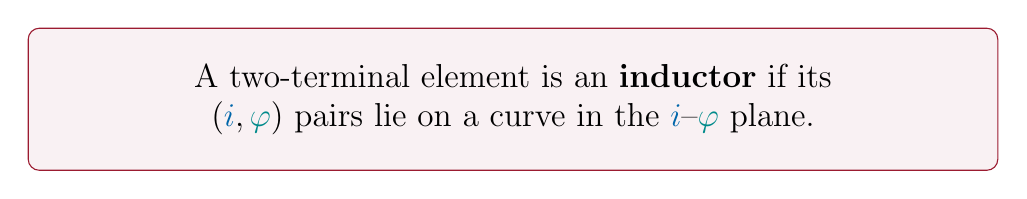
\begin{tikzpicture}
      \node[draw=metured, fill=metured!6, rounded corners=4pt, inner sep=13pt,
            text width=11.4cm, align=center, font=\large]
      {A two-terminal element is an \textbf{inductor} if its
       $(\Icol{i},\Fcol{\varphi})$ pairs lie on a
       \alert{curve in the $\Icol{i}$--$\Fcol{\varphi}$ plane}.};
    \end{tikzpicture}
  \end{center}
  \vfill
  \begin{center}
  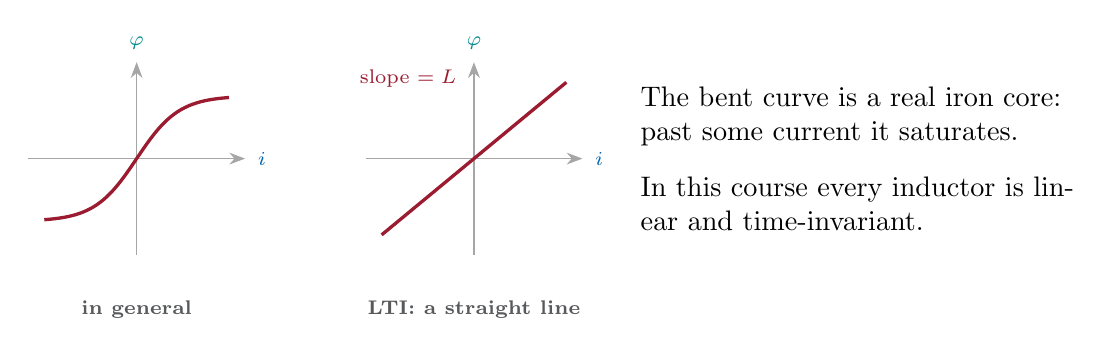
\begin{tikzpicture}[scale=1.02, transform shape]
    \begin{scope}
      \iphiaxes{1.35}{1.2}{in general}
      \draw[crv, domain=-1.15:1.15, samples=140, smooth] plot (\x, {0.78*tanh(1.9*\x)});
    \end{scope}
    \begin{scope}[xshift=4.2cm]
      \iphiaxes{1.35}{1.2}{LTI: a straight line}
      \draw[crv] (-1.15,-0.95) -- (1.15,0.95);
      \node[font=\scriptsize, text=metured] at (-0.82,1.0) {slope $=L$};
    \end{scope}
    \node[font=\normalsize, anchor=west, text width=5.5cm] at (6.15,0)
      {The bent curve is a real iron core: past some current it \alert{saturates}.\\[8pt]
       In this course every inductor is \alert{linear and time-invariant}.};
  \end{tikzpicture}
  \end{center}
  \vfill
\end{frame}

%--------------------------------------------------------------
\begin{frame}{And again, note what has \emph{not} happened}
  \vfill
  \begin{center}
    {\large An inductor has \alert{no characteristic} in the
     $\Vcol{v}$--$\Icol{i}$ plane either.}
  \end{center}
  \vfill
  \begin{center}
  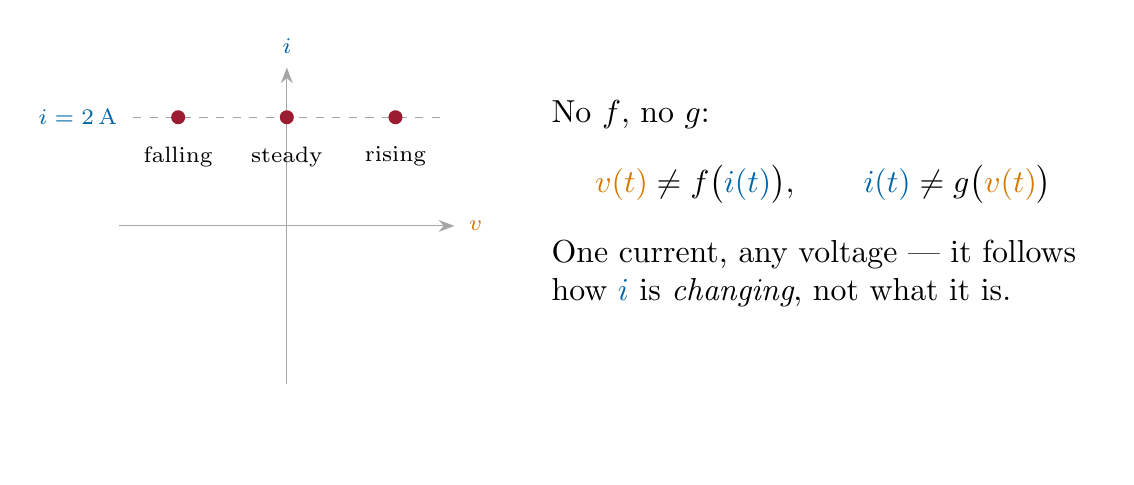
\begin{tikzpicture}[scale=1.15, transform shape]
    \viaxes{1.85}{1.75}{}
    \draw[metugray!55, dashed] (-1.7,1.2) -- (1.7,1.2);
    \node[font=\scriptsize, text=ccur, left] at (-1.75,1.2) {$\Icol{i} = 2\A$};
    \fill[metured] (1.2,1.2) circle (2.2pt);
    \fill[metured] (0,1.2) circle (2.2pt);
    \fill[metured] (-1.2,1.2) circle (2.2pt);
    \node[font=\scriptsize, below] at (1.2,1.0) {rising};
    \node[font=\scriptsize, below] at (0,1.0) {steady};
    \node[font=\scriptsize, below] at (-1.2,1.0) {falling};
    \node[font=\normalsize, anchor=west, text width=6.0cm] at (2.8,0.25)
      {No $f$, no $g$:
       \[ \Vcol{v(t)} \neq f\bigl(\Icol{i(t)}\bigr), \qquad
          \Icol{i(t)} \neq g\bigl(\Vcol{v(t)}\bigr) \]
       One current, \alert{any} voltage --- it follows how $\Icol{i}$ is
       \emph{changing}, not what it is.};
  \end{tikzpicture}
  \end{center}
  \vfill
\end{frame}

%--------------------------------------------------------------
\begin{frame}{The LTI inductor}
  \vfill
  \begin{center}
    {\large $\Fcol{\varphi} = L\,\Icol{i}$ --- a straight line whose slope is the
     \alert{same $L$} we met three slides ago. Differentiate:}
  \end{center}
  \vfill
  \begin{center}
  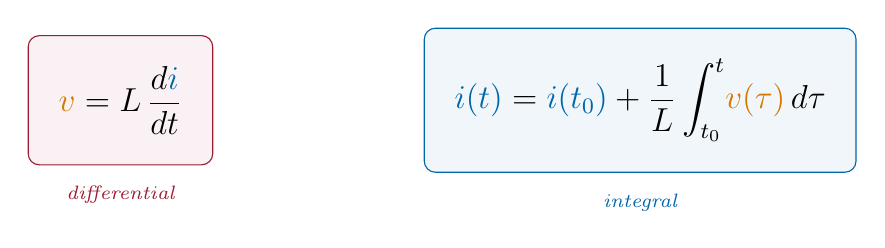
\begin{tikzpicture}[scale=1.0]
    \node[draw=metured, fill=metured!6, rounded corners=4pt, inner sep=11pt] (a) at (0,0)
      {\large $\displaystyle \Vcol{v} = L\,\frac{d\Icol{i}}{dt}$};
    \node[draw=ccur, fill=ccur!6, rounded corners=4pt, inner sep=11pt] (b) at (6.6,0)
      {\large $\displaystyle \Icol{i(t)} = \Icol{i(t_0)}
        + \frac{1}{L}\int_{t_0}^{t}\!\Vcol{v(\tau)}\,d\tau$};
    \node[font=\scriptsize\itshape, text=metured, below=4pt of a] {differential};
    \node[font=\scriptsize\itshape, text=ccur, below=4pt of b] {integral};
  \end{tikzpicture}
  \end{center}
  \vfill
  \begin{center}
    The voltage is whatever the \alert{rate of change} of current demands.\\
    The current is the \alert{running total} of everything the voltage has done.
  \end{center}
  \vfill
\end{frame}

%--------------------------------------------------------------
\begin{frame}{Four things that follow}
  \vfill
  \begin{columns}[T,onlytextwidth]
    \begin{column}{0.235\textwidth}
      \begin{block}{Short at DC}
        \small $\Icol{i}$ constant $\Rightarrow \frac{d\Icol{i}}{dt} = 0
        \Rightarrow \Vcol{v}=0$.
      \end{block}
    \end{column}
    \begin{column}{0.235\textwidth}
      \begin{block}{Current is continuous}
        \small Flip a switch, step the source: $\Icol{i}$ is the \emph{same} just after as
        just before. It always takes time to change.
      \end{block}
    \end{column}
    \begin{column}{0.235\textwidth}
      \begin{block}{It remembers}
        \small $\Icol{i(t)}$ depends on the \emph{whole history} of $\Vcol{v}$.
      \end{block}
    \end{column}
    \begin{column}{0.235\textwidth}
      \begin{block}{It holds energy}
        \small $\Pcol{w} = \tfrac12 L\Icol{i}^{\,2}$, set by the present current.
      \end{block}
    \end{column}
  \end{columns}
  \vfill
  \begin{center}
    {\large To a DC source, an inductor is just \alert{a piece of wire}.}
  \end{center}
  \vfill
\end{frame}

%--------------------------------------------------------------
\begin{frame}{Example: hold a constant voltage across it}
  \vfill
  \begin{center}
    $\Vcol{V} = 5\V$ across $L = 10\uni{mH}$, from $\Icol{i(0)} = 0$
    \qquad
    \onslide<2->{$\displaystyle \Icol{i(t)} = \frac{\Vcol{V}}{L}\,t = 500\,t$ \ [A]}
  \end{center}
  \vfill
  \begin{center}
  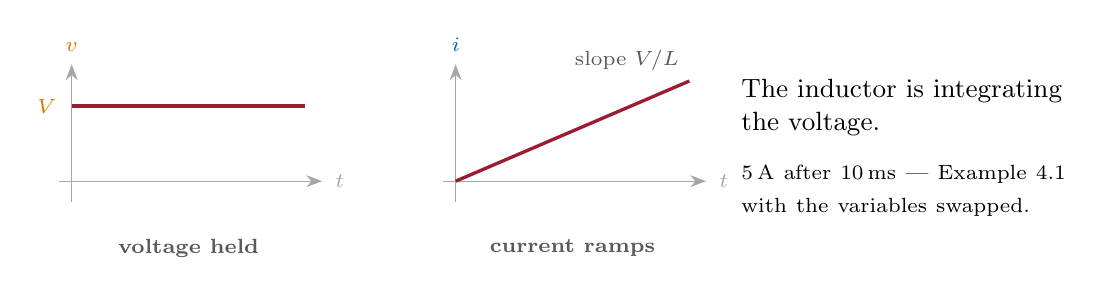
\begin{tikzpicture}[scale=1.06, transform shape]
    \begin{scope}
      \taxes{3.0}{0.25}{1.4}{\Vcol{$v$}}
      \draw[crv] (0,0.9) -- (2.8,0.9);
      \node[font=\scriptsize, text=cvolt, left] at (-0.06,0.9) {$V$};
      \node[ttl] at (1.4,-0.8) {voltage held};
    \end{scope}
    \begin{scope}[xshift=4.6cm]
      \taxes{3.0}{0.25}{1.4}{\Icol{$i$}}
      \draw[crv, visible on=<2->] (0,0) -- (2.8,1.2);
      \node[font=\scriptsize, text=metugray, above left, visible on=<2->]
           at (2.8,1.2) {slope $V/L$};
      \node[ttl, visible on=<2->] at (1.4,-0.8) {current ramps};
    \end{scope}
    \node[font=\small, anchor=west, text width=3.9cm, visible on=<3->] at (7.9,0.4)
      {The inductor is \alert{integrating} the voltage.\\[6pt]
       {\scriptsize $5\A$ after $10\uni{ms}$ --- Example 4.1 with the variables swapped.}};
  \end{tikzpicture}
  \end{center}
  \vfill
\end{frame}

%--------------------------------------------------------------
\begin{frame}{What if you try to stop the current?}
  \vspace{0.4em}
  \begin{columns}[T,onlytextwidth]
    \begin{column}{0.46\textwidth}
      \vspace{1.0em}
      \begin{center}
      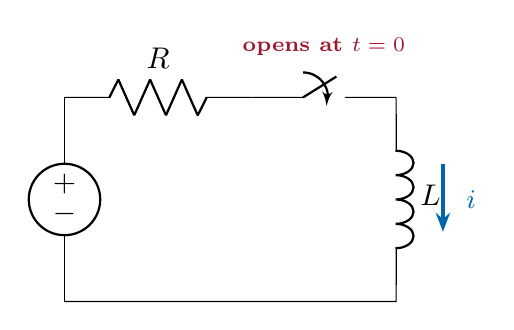
\begin{tikzpicture}[scale=1.08, transform shape]
        \draw (0,0) to[american voltage source, invert] (0,2.4);
        \draw (0,2.4) to[R, l=$R$] (2.2,2.4);
        \draw (2.2,2.4) to[cspst] (3.9,2.4);
        \node[font=\scriptsize\bfseries, text=metured] at (3.05,3.0) {opens at $t=0$};
        \draw (3.9,2.4) to[L, l=$L$] (3.9,0) -- (0,0);
        \draw[iar] (4.45,1.62) -- (4.45,0.82);
        \node[ccur, font=\small] at (4.78,1.2) {$\Icol{i}$};
      \end{tikzpicture}
      \end{center}
    \end{column}
    \begin{column}{0.50\textwidth}
      \vspace{0.6em}
      A steady $\Icol{i} = I_0$ is flowing.\\[12pt]
      \onslide<2->{The switch opens: $\Icol{i}$ must reach \alert{zero at once}.\\[12pt]}
      \onslide<3->{$\dfrac{d\Icol{i}}{dt} \to -\infty$, \ so
        $\Vcol{v} = L\,\dfrac{d\Icol{i}}{dt} \to -\infty$.}
    \end{column}
  \end{columns}
  \vspace{0.8em}
  \begin{center}
    \onslide<4->{{\large The inductor will do \alert{whatever it takes} to keep the current
      going ---}\\[4pt]
      so the voltage climbs until the \alert{air breaks down}, and $\tfrac12 L I_0^2$
      crosses the gap as a spark.}
  \end{center}
\end{frame}

%--------------------------------------------------------------
\begin{frame}{Where does the energy go?}
  \vfill
  \begin{center}
    {\large Raise $\Icol{i}$ from zero. The inductor pushes \alert{back}, so the circuit does
     \alert{work}.}
  \end{center}
  \vfill
  \begin{center}
    {\large $\displaystyle \Pcol{p} = \Vcol{v}\,\Icol{i} = L\,\Icol{i}\,\frac{d\Icol{i}}{dt}
      \qquad\onslide<2->{\Longrightarrow\qquad \int_0^{I}\! L\,\Icol{i}\,d\Icol{i}}$}
  \end{center}
  \vfill
  \begin{center}
    \onslide<3->{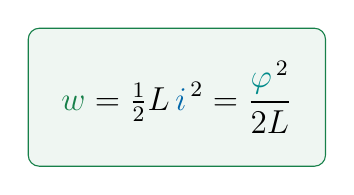
\begin{tikzpicture}
      \node[draw=cpow, fill=cpow!7, rounded corners=4pt, inner sep=12pt]
      {\large $\displaystyle \Pcol{w} = \tfrac12 L\,\Icol{i}^{\,2}
        = \frac{\Fcol{\varphi}^{\,2}}{2L}$};
    \end{tikzpicture}}
  \end{center}
  \vfill
  \begin{center}
    \onslide<3->{No resistance anywhere --- so none of it became heat.}
  \end{center}
  \vfill
\end{frame}

%--------------------------------------------------------------
\begin{frame}{Now run it backwards}
  \vfill
  \begin{center}
  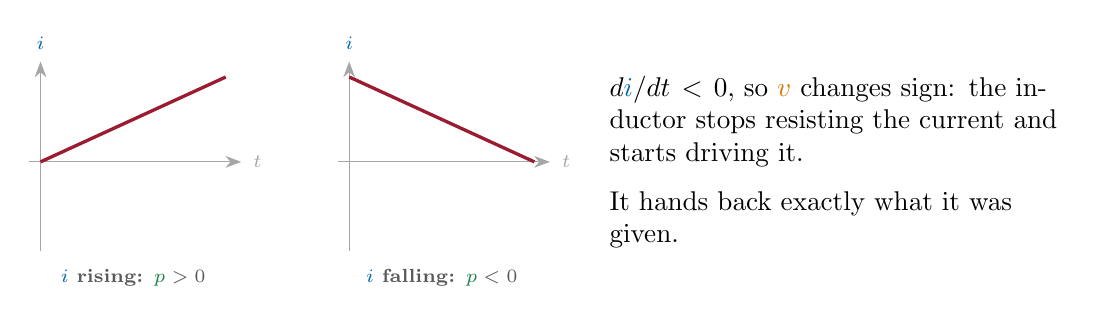
\begin{tikzpicture}[scale=0.98, transform shape]
    \begin{scope}
      \taxes{2.6}{1.15}{1.3}{\Icol{$i$}}
      \draw[crv] (0,0) -- (2.4,1.1);
      \node[ttl] at (1.2,-1.5) {$\Icol{i}$ rising: $\Pcol{p} > 0$};
    \end{scope}
    \begin{scope}[xshift=4.0cm]
      \taxes{2.6}{1.15}{1.3}{\Icol{$i$}}
      \draw[crv] (0,1.1) -- (2.4,0);
      \node[ttl] at (1.2,-1.5) {$\Icol{i}$ falling: $\Pcol{p} < 0$};
    \end{scope}
    \node[font=\normalsize, anchor=west, text width=6.0cm] at (7.25,0)
      {$d\Icol{i}/dt < 0$, so $\Vcol{v}$ changes sign: the inductor stops resisting the
       current and starts \alert{driving} it.\\[6pt]
       It hands back exactly what it was given.};
  \end{tikzpicture}
  \end{center}
  \vfill
  \begin{center}
    {\large $\Pcol{w} \ge 0$ always $\Rightarrow$ \alert{passive}. \quad
     Nothing lost either way $\Rightarrow$ \alert{lossless}.}\\[6pt]
    {\small Example: opening that switch was this handover done all at once --- as a spark.}
  \end{center}
  \vfill
\end{frame}

%--------------------------------------------------------------
\begin{frame}{So where was it kept?}
  \vfill
  \begin{center}
  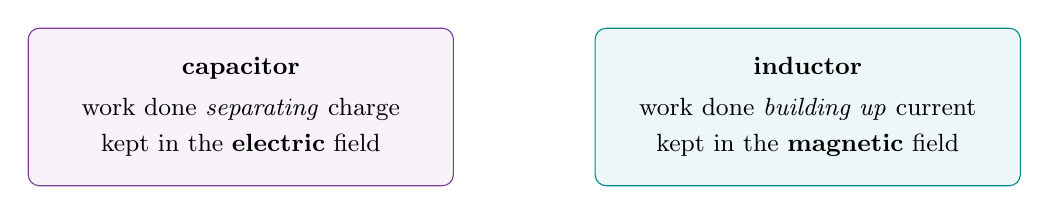
\begin{tikzpicture}[scale=1.0]
    \node[draw=ccharge, fill=ccharge!6, rounded corners=4pt, minimum width=5.4cm,
          minimum height=2.0cm, align=center, font=\small] (a) at (0,0)
         {\textbf{capacitor}\\[4pt] work done \emph{separating} charge\\[2pt]
          kept in the \textbf{electric} field};
    \node[draw=cflux, fill=cflux!7, rounded corners=4pt, minimum width=5.4cm,
          minimum height=2.0cm, align=center, font=\small] (b) at (7.2,0)
         {\textbf{inductor}\\[4pt] work done \emph{building up} current\\[2pt]
          kept in the \textbf{magnetic} field};
  \end{tikzpicture}
  \end{center}
  \vfill
  \begin{center}
    Not in the wire, and not in the moving charge --- in the \alert{field} around it.\\[6pt]
    {\large A field holds energy without consuming any.}\\[4pt]
    That is the whole reason these two are lossless and a resistor is not.
  \end{center}
  \vfill
\end{frame}

%--------------------------------------------------------------
\begin{frame}{For the mechanically minded}
  \vfill
  \begin{center}
    {\Large $\displaystyle \Vcol{v} = L\,\frac{d\Icol{i}}{dt}
      \qquad\longleftrightarrow\qquad u = \frac{1}{k}\,\frac{dF}{dt}$}
  \end{center}
  \vfill
  \begin{center}
  \small
  \begin{tabular}{@{}l c l@{}}
    \toprule
    \textbf{circuit} & & \textbf{mechanical}\\
    \midrule
    current $\Icol{i}$        & $\leftrightarrow$ & force $F$\\
    voltage $\Vcol{v}$        & $\leftrightarrow$ & velocity $u$\\
    capacitance $C$           & $\leftrightarrow$ & mass $m$ \quad {\scriptsize(Lecture 4)}\\
    inductance $L$            & $\leftrightarrow$ & spring compliance $1/k$\\
    $\tfrac12 L\Icol{i}^{\,2}$ & $\leftrightarrow$ & $F^2/2k$\\
    \bottomrule
  \end{tabular}
  \end{center}
  \vfill
  \begin{center}
    A \alert{stiff} spring is a \alert{small} inductance.
  \end{center}
  \vfill
\end{frame}

%--------------------------------------------------------------
\begin{frame}{The three LTI elements, side by side}
  \vfill
  \begin{center}
  \footnotesize
  \renewcommand{\arraystretch}{1.15}
  \begin{tabular}{@{}l l l l@{}}
    \toprule
     & \textbf{LTI resistor} & \textbf{LTI capacitor} & \textbf{LTI inductor}\\
    \midrule
    characteristic in  & $\Vcol{v}$--$\Icol{i}$ & $\Vcol{v}$--$\Qcol{q}$ & $\Icol{i}$--$\Fcol{\varphi}$\\
    that characteristic& $\Vcol{v} = R\Icol{i}$ & $\Qcol{q} = C\Vcol{v}$ & $\Fcol{\varphi} = L\Icol{i}$\\
    terminal equation  & $\Vcol{v} = R\Icol{i}$ & $\Icol{i} = C\,d\Vcol{v}/dt$ & $\Vcol{v} = L\,d\Icol{i}/dt$\\
    unit               & ohm, $\Omega$ & farad, F & henry, H\\
    memory             & none & the past of $\Icol{i}$ & the past of $\Vcol{v}$\\
    at DC it is        & itself & an \emph{open} circuit & a \emph{short} circuit\\
    cannot jump        & --- & its voltage & its current\\
    energy $\Pcol{w}$  & --- & $\tfrac12 C\Vcol{v}^{\,2}$ & $\tfrac12 L\Icol{i}^{\,2}$\\
    verdict            & passive, \emph{lossy} & passive, \emph{lossless} & passive, \emph{lossless}\\
    \bottomrule
  \end{tabular}
  \end{center}
  \vfill
  \begin{center}
    Swap $\Vcol{v}\leftrightarrow\Icol{i}$, $\Qcol{q}\leftrightarrow\Fcol{\varphi}$,
    $C\leftrightarrow L$ and the last two columns \alert{turn into each other}.
  \end{center}
  \vfill
\end{frame}

%--------------------------------------------------------------
\begin{frame}{A circuit with all three}
  \vspace{-0.2em}
  \begin{center}
  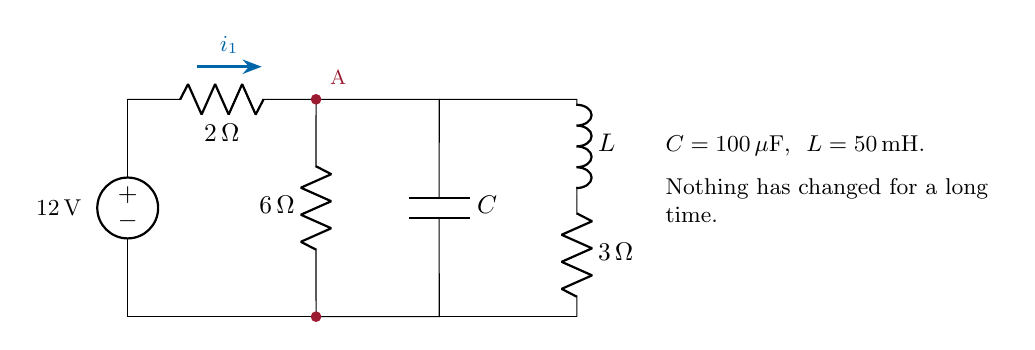
\begin{tikzpicture}[scale=0.92, transform shape]
    \draw (0,0) to[american voltage source, invert] (0,3.0);
    \node[font=\small] at (-0.95,1.5) {$12\V$};
    \draw (0,3.0) to[R, l_=$2\ohm$] (2.6,3.0);
    \draw[iar] (0.95,3.45) -- (1.85,3.45);
    \node[ccur, font=\small] at (1.4,3.75) {$i_1$};
    \draw (2.6,3.0) to[R, l_=$6\ohm$] (2.6,0);
    \draw (2.6,3.0) -- (4.3,3.0) to[C, l=$C$] (4.3,0) -- (2.6,0);
    \draw (4.3,3.0) -- (6.2,3.0) to[L, l=$L$] (6.2,1.7);
    \draw (6.2,1.7) to[R, l=$3\ohm$] (6.2,0);
    \draw (6.2,0) -- (0,0);
    \node[gnode] at (2.6,3.0) {};
    \node[gnode] at (2.6,0) {};
    \node[glab, above right=1pt and 2pt] at (2.6,3.05) {A};
    \node[font=\small, anchor=west, text width=4.6cm] at (7.3,1.9)
      {$C = 100\uni{\mu F}$, \ $L = 50\uni{mH}$.\\[6pt]
       Nothing has changed for a long time.};
  \end{tikzpicture}
  \end{center}
  \vspace{-0.1em}
  \begin{center}
    \onslide<1>{{\large\color{metured} Every branch voltage and current $=$ ?}}
  \end{center}
  \begin{center}
    \onslide<2->{{\large Every derivative is zero, so by the table:
      $C$ is an \alert{open circuit}, $L$ is a \alert{short circuit}.}\\[3pt]
      What is left is Lecture 2's resistive circuit.}
  \end{center}
\end{frame}

%--------------------------------------------------------------
\begin{frame}{The steady state, solved}
  \vspace{-0.2em}
  \begin{center}
  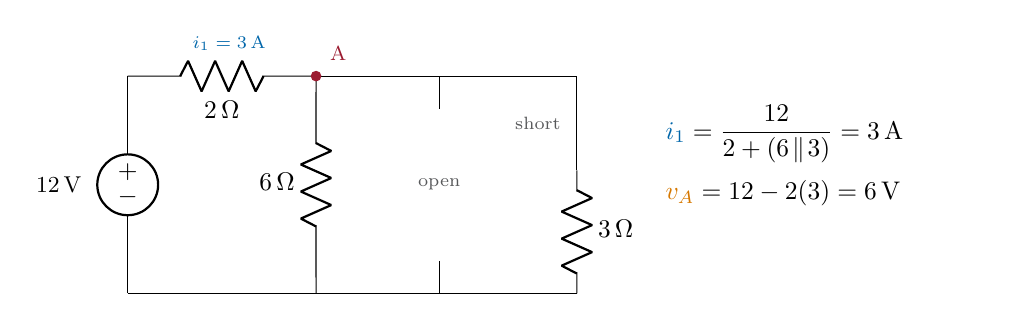
\begin{tikzpicture}[scale=0.92, transform shape]
    \draw (0,0) to[american voltage source, invert] (0,3.0);
    \node[font=\small] at (-0.95,1.5) {$12\V$};
    \draw (0,3.0) to[R, l_=$2\ohm$] (2.6,3.0);
    \draw (2.6,3.0) to[R, l_=$6\ohm$] (2.6,0);
    \draw (2.6,3.0) -- (4.3,3.0) -- (4.3,2.55);
    \node[font=\scriptsize, text=metugray] at (4.3,1.5) {open};
    \draw (4.3,0.45) -- (4.3,0) -- (2.6,0);
    \draw (4.3,3.0) -- (6.2,3.0) -- (6.2,1.7);
    \draw (6.2,1.7) to[R, l=$3\ohm$] (6.2,0);
    \draw (6.2,0) -- (0,0);
    \node[font=\scriptsize, text=metugray, left] at (6.1,2.35) {short};
    \node[gnode] at (2.6,3.0) {};
    \node[glab, above right=1pt and 2pt] at (2.6,3.05) {A};
    \node[ccur, font=\scriptsize] at (1.4,3.45) {$i_1 = 3\A$};
    \node[font=\normalsize, anchor=west, text width=4.6cm] at (7.3,1.9)
      {$\displaystyle \Icol{i_1} = \frac{12}{2 + (6\!\parallel\!3)} = 3\A$\\[6pt]
       $\Vcol{v_A} = 12 - 2(3) = 6\V$};
  \end{tikzpicture}
  \end{center}
  \vspace{-0.1em}
  \begin{center}\small
    $\Icol{i_{6\Omega}} = 1\A$, \quad $\Icol{i_L} = \Icol{i_{3\Omega}} = 2\A$, \quad
    $\Vcol{v_C} = 6\V$, \quad $\Vcol{v_L} = 0$, \quad $\Icol{i_C} = 0$.\\[4pt]
    Stored: \ $\Pcol{w_C} = \tfrac12(10^{-4})(6)^2 = 1.8\uni{mJ}$, \quad
    $\Pcol{w_L} = \tfrac12(0.05)(2)^2 = 0.1\J$.
  \end{center}
\end{frame}

%--------------------------------------------------------------
\begin{frame}{Where is the power going?}
  \vfill
  \begin{center}
  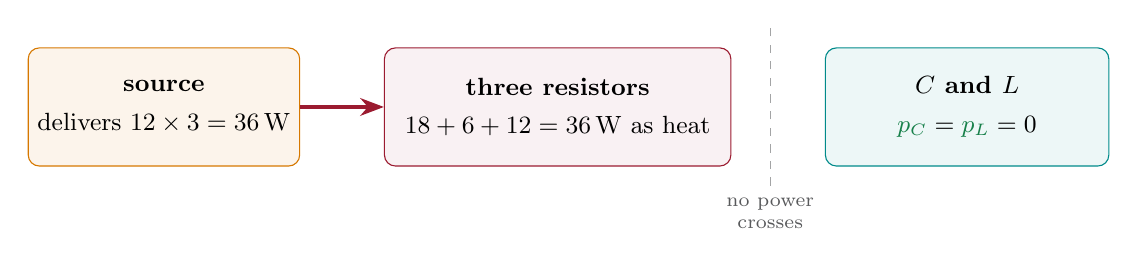
\begin{tikzpicture}[scale=1.0]
    \node[draw=cvolt, fill=cvolt!8, rounded corners=4pt, minimum width=3.3cm,
          minimum height=1.5cm, align=center, font=\small] (s) at (0,0)
         {\textbf{source}\\[3pt] delivers $12\times 3 = 36\W$};
    \node[draw=metured, fill=metured!6, rounded corners=4pt, minimum width=4.4cm,
          minimum height=1.5cm, align=center, font=\small] (r) at (5.0,0)
         {\textbf{three resistors}\\[3pt] $18 + 6 + 12 = 36\W$ as heat};
    \node[draw=cflux, fill=cflux!7, rounded corners=4pt, minimum width=3.6cm,
          minimum height=1.5cm, align=center, font=\small, visible on=<2->] (cl) at (10.2,0)
         {\textbf{$C$ and $L$}\\[3pt] $\Pcol{p_C} = \Pcol{p_L} = 0$};
    \draw[flowarr] (s) -- (r);
    \draw[metugray!55, dashed, visible on=<2->] (7.7,-1.0) -- (7.7,1.0);
    \node[font=\scriptsize, text=metugray, visible on=<2->, align=center] at (7.7,-1.35)
         {no power\\ crosses};
  \end{tikzpicture}
  \end{center}
  \vfill
  \begin{center}
    \onslide<2->{$\Pcol{p_C} = \Vcol{v_C}\Icol{i_C} = 6\times 0 = 0$, \qquad
      $\Pcol{p_L} = \Vcol{v_L}\Icol{i_L} = 0\times 2 = 0$.\\[6pt]
      {\large They \alert{hold} energy. They do not consume any.}}
  \end{center}
  \vfill
\end{frame}

%--------------------------------------------------------------
\begin{frame}{Summary}
  \vfill
  \begin{itemize}\itemsep5pt
    \item An \textbf{inductor} fights changes in current. Integrate the voltage:
          $\Fcol{\varphi} = \int\!\Vcol{v}\,d\tau$ in \textbf{volt-seconds} (webers), as
          charge was amp-seconds. An \textbf{inductor} is a curve in the
          $\Icol{i}$--$\Fcol{\varphi}$ plane --- not a resistor.
    \item \textbf{LTI inductor}: $\Vcol{v} = L\,d\Icol{i}/dt$, or the integral form. Short
          circuit at DC; current cannot jump; it remembers.
    \item \textbf{Inductance} $L$ in henries --- set by the turn count, the winding's
          shape and what is inside it. One henry is large.
    \item Starting the current means \textbf{work against} that opposing voltage:
          $\Pcol{w} = \tfrac12 L\Icol{i}^{\,2}$, kept in the \alert{magnetic field} and
          handed back in full. Forcing the current to jump demands a voltage impulse ---
          in a real switch, a spark.
    \item In a \textbf{DC steady state}: $C$ open, $L$ short, and neither absorbs power.
  \end{itemize}
  \vfill
\end{frame}

%--------------------------------------------------------------
\begin{frame}{Next lecture}
  \vfill
  \begin{center}
  \begin{block}{Dependent sources}
    Sources whose value is set by a voltage or a current \emph{somewhere else} in the
    circuit --- how a transistor or an op-amp gets into a circuit diagram.
  \end{block}
  \end{center}
  \vfill
  \begin{center}
    {\Large\color{metured} Questions?}\\[8pt]
    {\small Notes for this lecture: see the course repository.}
  \end{center}
  \vfill
\end{frame}

\end{document}
